\chapter{A primer in urban form}\label{ch:primer}

\section{What urban form is}
\input{generated/nb_urban_form_2}

\section{Three street patterns}
Most street networks are mixtures of three ideal patterns (Figure~\ref{fig:patterns}). Keep them in mind: each measure in the next chapters separates them in a different way.

\begin{figure}[H]\centering
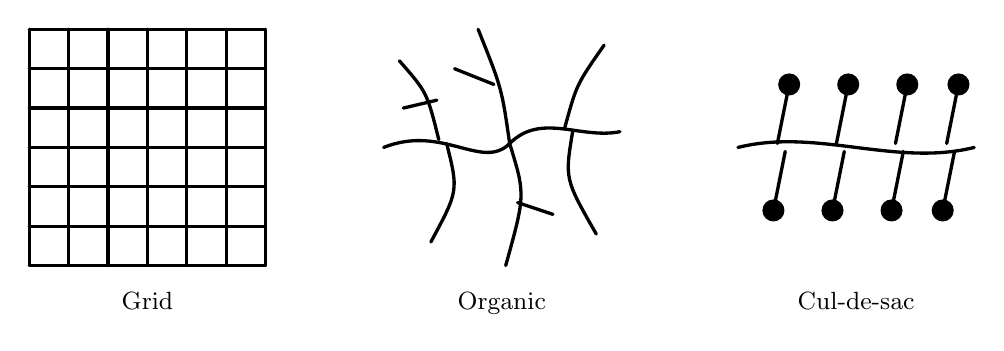
\begin{tikzpicture}[x=0.5cm,y=0.5cm, line width=1.2pt, line cap=round]
  % grid
  \foreach \i in {0,...,6} { \draw (\i,0) -- (\i,6); \draw (0,\i) -- (6,\i); }
  \node[below, font=\small] at (3,-0.4) {Grid};
  % organic
  \begin{scope}[xshift=4.5cm]
    \draw (0,3) .. controls (1.5,3.6) and (2.5,2.4) .. (3.2,3.1) .. controls (4,3.9) and (5,3.2) .. (6,3.4);
    \draw (3.2,3.1) .. controls (3,4.5) .. (2.4,6);
    \draw (3.2,3.1) .. controls (3.6,1.8) .. (3.1,0);
    \draw (1.4,3.2) .. controls (1.1,4.4) .. (0.4,5.2);
    \draw (1.6,3.1) .. controls (1.9,1.9) .. (1.2,0.6);
    \draw (4.6,3.5) .. controls (4.9,4.6) .. (5.6,5.6);
    \draw (4.8,3.4) .. controls (4.6,2.2) .. (5.4,0.8);
    \draw (2.8,4.6) -- (1.8,5.0); \draw (3.4,1.6) -- (4.3,1.3); \draw (1.35,4.2) -- (0.5,4.0);
    \node[below, font=\small] at (3,-0.4) {Organic};
  \end{scope}
  % cul-de-sac
  \begin{scope}[xshift=9cm]
    \draw (0,3) .. controls (2,3.5) and (4,2.5) .. (6,3);
    \foreach \x/\d in {1/1,2.5/1,4/1,5.3/1} {
      \draw (\x,3.1) -- (\x+0.3,4.6); \fill (\x+0.3,4.6) circle (0.28);
      \draw (\x+0.2,2.9) -- (\x-0.1,1.4); \fill (\x-0.1,1.4) circle (0.28);
    }
    \node[below, font=\small] at (3,-0.4) {Cul-de-sac};
  \end{scope}
\end{tikzpicture}
\caption{Three ideal street patterns. The grid has many four-way junctions, two dominant directions and short, direct routes. The organic pattern, grown over time, has three-way junctions, every direction and moderately direct routes. The cul-de-sac pattern feeds dead ends from a curving distributor road: few junctions and long, indirect routes on foot unless footpaths cut through.}\label{fig:patterns}
\end{figure}

The grid is old: Hippodamus of Miletus planned one in the fifth century BC, Roman camps were grids, and so are Mohenjo-daro, Manhattan and Cerd\`a's Barcelona. Organic fabrics grow plot by plot along paths and are typical of pre-modern cores such as Lahore's Walled City. The cul-de-sac layout belongs to twentieth-century planning that separated cars from homes, as in new towns like Craigavon. None is simply good or bad: grids are legible and easy to walk but can carry through-traffic everywhere; cul-de-sacs are quiet but make short trips long.

\section{Getting the data}
\input{generated/nb_urban_form_3}

The measures in this guide follow published methods: OSMnx for building and measuring networks \citep{Boeing_2017,Boeing_2018}, street orientation entropy \citep{Boeing_2019}, the Spacematrix for density \citep{BerghauserPont_2010}, and momepy for building morphometrics \citep{Fleischmann_2019}. The layered reading of the town plan goes back to \citet{Conzen_1960}, and the study of street configuration to \citet{Hillier_1984}.
